\taughtsession{Lecture}{Syntax Analysis and Parsing}{2024-02-19}{1400}{Jiacheng}{}

\section{Ambiguities in Grammars}
Unsurprisingly, given the complex and custom nature of grammars - it is possible to make them ambiguous. This would mean that the derivation of given sentences could be different, therefore the parse trees are different.\\

For example if we take a left-most derivation for the sentence \verb|x + y * z|:
\begin{lstlisting}
    <exp> $\Rightarrow$ <exp> + <exp>
          $\Rightarrow$ x + <exp>
          $\Rightarrow$ x + <exp> * <exp>
          $\Rightarrow$ x + y * <exp>
          $\Rightarrow$ x + y * z
\end{lstlisting}
However, we can first apply the rule:
\begin{lstlisting}
    <exp> $\rightarrow$ <exp> * <exp>
\end{lstlisting}
which would yield:
\begin{lstlisting}
    <exp> $\Rightarrow$ <exp> * <exp>
          $\Rightarrow$ <exp> + <exp> * <exp>
          $\Rightarrow$ x + <exp> * <exp>
          $\Rightarrow$ x + y * <exp>
          $\Rightarrow$ x + y * z
\end{lstlisting}

These two derivations would produce different parse trees:
\begin{figure}[H]
\centering
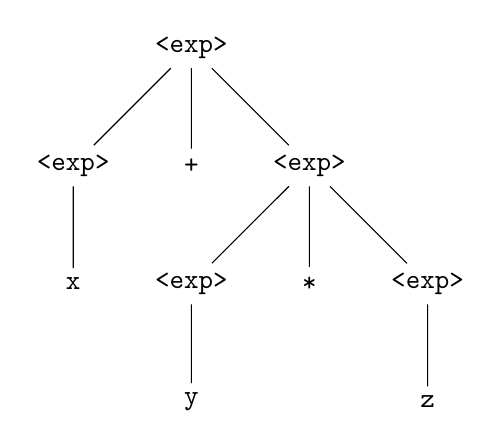
\begin{tikzpicture}[font=\ttfamily]
\node{<exp>}   
    child {node {<exp>}
        child {node {x}}}   
    child {node {+}}
    child {node {<exp>}
        child {node{<exp>}
            child {node {y}}}
        child {node {*}}
        child {node{<exp>}
            child {node{z}}}
    };
\end{tikzpicture}
\caption{Parse Tree for derivation of \texttt{x + y * z}}
\end{figure}

\begin{figure}[H]
\centering
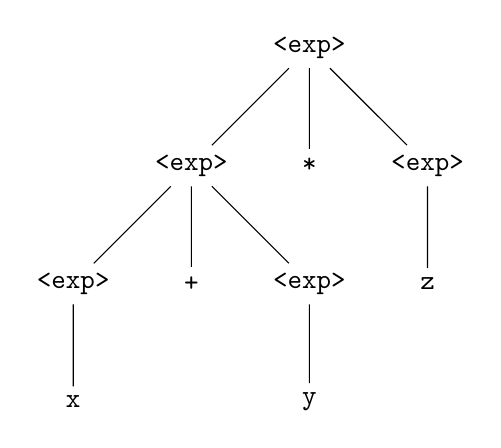
\begin{tikzpicture}[font=\ttfamily]
\node{<exp>}   
    child {node {<exp>}
        child {node{<exp>}
            child {node {x}}}
        child {node {+}}
        child {node{<exp>}
        child {node{y}}}}
    child {node {*}}
    child {node {<exp>}
        child {node {z}} 
    };
\end{tikzpicture}
\caption{Parse Tree for alternate derivation of \texttt{x + y * z}}
\end{figure}

An \textit{Abstract Syntax Tree} only shows the terminal symbols, without showing expressions. 

\begin{figure}[H]
\centering
\begin{tikzpicture}[font=\ttfamily]
\node{+}   
    child {node {x}}
    child {node {*}
        child {node {y}}
        child {node {z}}              
    };
\end{tikzpicture}
\caption{Example of an Abstract Syntax Tree}
\end{figure}
    

\subsection{Avoiding Ambiguity}
Ambiguity in grammars should be avoided, as we know from primary school - ambiguity in mathematical expressions has been removed through having an order of precedence which we can use brackets as part of.

\subsection{Removing Ambiguity}
For nearly all programming languages, the ambiguities in a grammar can be removed. To do this, extra non-terminals and rules are added. For example, taking the example grammar below:
\begin{lstlisting}
    <exp> $\rightarrow$ <exp> + <exp> | <exp> * <exp> | x | y | z
\end{lstlisting}
which can be disambiguated by adding rules that force certain operations (\verb|+|) to appear above other operators (\verb|*|) in parse trees. Thus giving the standard precedence of \verb|+| then \verb|*|. The new grammar can be seen below:
\begin{lstlisting}
       <exp> $\rightarrow$ <exp> + <term> | <term>
      <term> $\rightarrow$ <term> * <factor> | <factor>
    <factor> $\rightarrow$ x | y | z
\end{lstlisting}
Note that \verb|term| and \verb|factor| are newly introduced non-terminals.

\subsection{Limits of Context-Free Grammars}
There are some aspects of programming language syntax that cannot be captured using a context-free grammar. For example, the rule that variables must be declared before they are used is a \textit{context sensitive} property. Context-sensitive properties are resolved by the semantic analyser (which is beyond the scope of this module). 

\section{Syntax Analyser}
For any given input program, the goals of syntax analysis (also known as parsing) are to:
\begin{itemize}
    \item find all syntax errors, and for each discovered - produce an appropriate diagnostic message and recover quickly
    \item produce the parse tree for the program for code generation
\end{itemize}
These two functions are carried out by the syntax analyser (also known as the parser). There are different algorithms for parsing which are completed by different parsers.

\subsection{An Example}
If we take the grammar:
\begin{lstlisting}
    <exp> $\rightarrow$ <exp> + <exp> | <exp> * <exp> | x | y | z
\end{lstlisting}
the source code:
\begin{verbatim}
    x + y * z
\end{verbatim}
It will produce the tokens outputted by the scanner:
\begin{verbatim}
    IDENT PLUS IDENT MULTI IDENT
\end{verbatim}
And the following Parse Tree:
\begin{figure}[H]
\centering
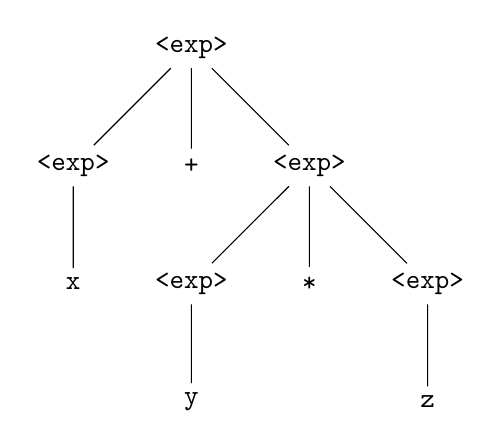
\begin{tikzpicture}[font=\ttfamily]
\node{<exp>}   
    child {node {<exp>}
        child {node {x}}}   
    child {node {+}}
    child {node {<exp>}
        child {node{<exp>}
            child {node {y}}}
        child {node {*}}
        child {node{<exp>}
            child {node{z}}}
    };
\end{tikzpicture}
\caption{Example Parse Tree for derivation of \texttt{x + y * z}}
\end{figure}
With the following abstract syntax tree:
\begin{figure}[H]
\centering
\begin{tikzpicture}[font=\ttfamily]
\node{+}   
    child {node {x}}
    child {node {*}
        child {node {y}}
        child {node {z}}              
    };
\end{tikzpicture}
\caption{AST For example}
\end{figure}

\section{Parsers}
There are two categories of parsers.\\

\textbf{Top-Down Parsers} begin with the root (the start symbol of the grammar rules) then visit each node (of the parse tree) before the branches are followed. For a left-most derivation, the branches from a given node are visited in left-to-right order.\\

\textbf{Bottom-Up Parsers} begin at the leaves of the parse tree (which are terminal symbols) and progress towards the root. The order is that of the reverse of a rightmost derivation.

\subsection{Parsing: An Example}
If we consider the following grammar:
\begin{align*}
    S & \rightarrow AB\\
    A & \rightarrow aA|\varepsilon \\
    B & \rightarrow b | bB
\end{align*}
The above grammar defines strings consisting of any number (0 included) of $a$'s followed by at least one (with the possibility of more) $b$'s. \\

If we consider parsing the string $aaab$ using the grammar by top-down parsing:
\begin{enumerate}
    \item begin with the start symbol $S$ and read the sentence one character at a time from the left
    \item at each step - expand the leftmost non-terminal by replacing it with the right side of one of its productions
    \item repeat until only terminals remain
\end{enumerate}
Shown below is the full parsing for the string:
\begin{itemize}
    \setlength{\itemindent}{2em}
    \item[$\boldsymbol{S}$] Begin with $S$ (start symbol)
    \item[$\boldsymbol{A}B$] $S \rightarrow AB$ (replace $S$ with the right hand side of $S \rightarrow AB$)
    \item[$a\boldsymbol{A}B$] $A \rightarrow aA$ (the leftmost non-terminal is $A$. On seeing first input $a$, replace $A$ with the right hand side of $A \rightarrow aA$)
    \item[$aa\boldsymbol{A}B$] $A\rightarrow aA$ (on seeing 2nd $a$)
    \item[$aaa\boldsymbol{A}B$] $A \rightarrow aA$ (on seeing 3rd $a$)
    \item[$aaa\varepsilon\boldsymbol{B}$] $A \rightarrow \varepsilon$ (on seeing $b$, use $A \rightarrow \varepsilon$ to make $A$ disappear as there is no rule for $A \rightarrow b$ and we can't work on non-terminal $B$ yet)   
    \item[$aaa\boldsymbol{B}$] 
    \item[$aaab$] $B \rightarrow b$ (on seeing $b$)
\end{itemize}

The top-down parse of the string $aaab$ is a left-most derivation of the sentence, which verifies that $aaab$ is a legal sentence. \\

At each step of top-down parsing:
\begin{itemize}
    \item Give a general sentential form, $xA\alpha$ where $x$ is a string of terminal symbols, $A$ is a non-terminal symbol and $\alpha$ is a mixed string of terminal \& non-terminal symbols. 
    \item THis means that $A$ is the leftmost non-terminal that must be expanded to get the next sentential form in a leftmost derivation. 
    \item Determining the next sentential form is a matter of choosing the correct grammar rule that has $A$ as its left hand side. 
\end{itemize}
For example, with the current sentential form, $xA\alpha$, suppose the grammar has three rules for A:
\begin{align*}
    A & \rightarrow bB\\
    A & \rightarrow cBb\\
    A & \rightarrow a
\end{align*}
Depending upon the next input being $a$, $b$ or $v$, a top-down parser must choose among these three rules to generate the nex sentential form (from $xA\alpha$). 

\subsection*{Predictive Parsers}
Different top-down parsing algorithms may use different information to make parsing decision (choosing the correct rules). Most parsers compare the next input token with the first symbols that can be generated by the right hand side of those rules, therefore called predictive parsers. A predictive parser is characterized by its ability to choose the production rule to apply solely based on the next input symbol and the current non-terminal being processed:
\begin{itemize}
    \item Current non-terminal $\Rightarrow$ chose the candidate rules
    \item Next input $\Rightarrow$ choose one rule among the candidates
\end{itemize}
Over this lecture and the next one, we will explore two different implementations of a predictive (top-down) parser.
\begin{itemize}
    \item Recursive descent parsers - a coded implementation of a syntax analyser based on BDF description of syntax
    \item LL (1) parsers - driven by a parsing table (created from BNF grammar) with: 1st L is a left-to-right scan of input; 2nd L is a leftmost derivation; and the `1' meaning one input symbol of lookahead (i.e. predictive)
\end{itemize}

\section{Recursive-Descent Parsers (RDP)}
A Recursive-Descent Parser (RDP) is made up of a collection of subprograms, many of which are recursive (hence where its name comes from) and produces a parse tree in top-down order.\\

Within an RDP - there is a subprogram for each non-terminal in the grammar. 

\subsection{RDP Example}
If we take the following grammar for a small set of simple expressions:
\begin{lstlisting}
       <exp> $\rightarrow$ <term> + <term> | <term> - <term>
      <term> $\rightarrow$ <factor> * <factor> | <factor> / <factor>
    <factor> $\rightarrow$ id | int_constant | (<exp>)
\end{lstlisting}

We can re-write the grammar for \verb|<exp>| and \verb|<term>| in a more compact form, because the only difference in the two alternatives in both cases is a terminal symbol (\verb|+| or \verb|-|, \verb|*| or \verb|/|):
\begin{lstlisting}
       <exp> $\rightarrow$ { ( + | - ) <term> }
      <term> $\rightarrow$ { ( * | / ) <factor> }
    <factor> $\rightarrow$ id | int_constant | (<exp>)
\end{lstlisting}

To implement a programmed recursive-descent parser, we need to implement three subprograms:
\begin{itemize}
    \item \verb|exp()|
    \item \verb|term()|
    \item \verb|factor()|
\end{itemize}
We would also assume that we have a lexical analyser (for example \verb|lex()|) that puts the next token in a variable called \verb|nextToken|. Upon receiving a token, the parser will decide:
\begin{itemize}
    \item if it is a terminal of current rule (i.e, \verb|+|, \verb|-|, \verb|*|, \verb|/|, \verb|id|, \ldots), continue to have the next token (make a call to \verb|lex()| to get \verb|nextToken|). 
    \item if it is a non-terminal symbol fo the right hand side of the current rule (i.e. \verb|<term>|, \verb|<factor>|), call it's associated parsing subprogram for that non-terminal
    \item if it is neither terminal nor non-terminal of the current rule or something else, then there is a syntax error.
\end{itemize}

\subsection{Rules with Multiple Right Hand Sides}
Where a rule ha multiple right hand sides, a decision has to be taken as to which one to use. The correct RHS could be chosen based on the next token of input - which is compared with the first token of each RHS until a match is found. If no match is found, it is a syntax error.